\subsection[CO binding energies]{\ce{CO} binding energies}

We next compare the \(BE_{\rm ad}(\ce{CO})\) values for the \ce{Pt10^{der}CO} and
\ce{Pt_xGe_{10-x}^{der}CO} series. We also examine the GM calculations to see
how the starting structure and multiplicity affect the binding energies. For each model, \ce{CO} was placed at
each unique Pt site. The labels in Supporting
Figure~\ref{fig:tfg_site_numbering} identify these initial unique placements.
Note that clusters are flexible, therefore different initial placements can relax to the same optimized carbonyl structure.

For \ce{Pt10^{der}}, the ten triplet sites give seven distinct
\ce{Pt10^{der}CO} minima, shown in Figure~\ref{fig:tfg_pt10co_series}.
The labels 1/9, 3/5, and 8/10 indicate that different initial positions lead
to the same optimized structure. The corresponding optimized structures for
\ce{Pt6Ge4^{der}CO}, \ce{Pt5Ge5^{der}CO}, and \ce{Pt4Ge6^{der}CO} are shown
in Figure~\ref{fig:tfg_ptgeco_series}.

\begin{figure}[H]
\centering
\begin{tikzpicture}[
  x=1cm,
  y=1cm,
  structure/.style={inner sep=0pt},
  sitelabel/.style={font=\sffamily\scriptsize, align=center},
  datalabel/.style={font=\sffamily\tiny, align=center, text=black!75}
]

% Global layout controls.
\def\molw{0.22\linewidth}
\def\rowone{1.75}
\def\rowtwo{-1.75}
\def\xone{-4.35}
\def\xtwo{-1.45}
\def\xthree{1.45}
\def\xfour{4.35}
\def\labelshift{-1.48cm}
\def\datashift{-1.77cm}

% Seven unique minima obtained from the ten original TFG starting sites.
\node[structure] (site1) at (\xone,\rowone)
  {\includegraphics[width=\molw]{Pt10CO/Pt1_from_1xyzUnai.png}};
\node[structure] (site2) at (\xtwo,\rowone)
  {\includegraphics[width=\molw]{Pt10CO/Pt2_from_2xyzUnai.png}};
\node[structure] (site5) at (\xthree,\rowone)
  {\includegraphics[width=\molw]{Pt10CO/Pt5_from_5xyzUnai.png}};
\node[structure] (site4) at (\xfour,\rowone)
  {\includegraphics[width=\molw]{Pt10CO/pt4_from_4xyzUnai.png}};

\node[structure] (site6) at (-4.0,\rowtwo)
  {\includegraphics[width=\molw]{Pt10CO/Pt6_from_6xyzUnai.png}};
\node[structure] (site7) at (0,\rowtwo)
  {\includegraphics[width=\molw]{Pt10CO/Pt7_from_7xyzUnai.png}};
\node[structure] (site8) at (4.0,\rowtwo)
  {\includegraphics[width=\molw]{Pt10CO/Pt8_from_8xyzUnai.png}};

% Starting-site labels and binding energies of the final minima.
\node[sitelabel] at ([yshift=\labelshift]site1.center) {Sites 1/9};
\node[datalabel] at ([yshift=\datashift]site1.center) {$-2.156$ eV};
\node[sitelabel] at ([yshift=\labelshift]site2.center) {Site 2};
\node[datalabel] at ([yshift=\datashift]site2.center) {$-2.493$ eV};
\node[sitelabel] at ([yshift=\labelshift]site5.center) {Sites 3/5};
\node[datalabel] at ([yshift=\datashift]site5.center) {$-2.590$ eV};
\node[sitelabel] at ([yshift=\labelshift]site4.center) {Site 4};
\node[datalabel] at ([yshift=\datashift]site4.center) {$-2.579$ eV};

\node[sitelabel] at ([yshift=\labelshift]site6.center) {Site 6};
\node[datalabel] at ([yshift=\datashift]site6.center) {$-2.657$ eV};
\node[sitelabel] at ([yshift=\labelshift]site7.center) {Site 7};
\node[datalabel] at ([yshift=\datashift]site7.center) {$-2.493$ eV};
\node[sitelabel] at ([yshift=\labelshift]site8.center) {Sites 8/10};
\node[datalabel] at ([yshift=\datashift]site8.center) {$-2.650$ eV};

\end{tikzpicture}

\caption{Seven distinct optimized triplet \ce{Pt10CO} structures obtained by
placing \ce{CO} at the ten Pt sites of \ce{Pt10^{der}}. The labels indicate the
initial adsorption sites; labels such as 1/9, 3/5, and 8/10 denote starting
sites that converge to the same optimized structure. The corresponding
$BE_{\rm ad}(\ce{CO})$ values are given below each structure.}
\label{fig:tfg_pt10co_series}
\end{figure}

The optimized carbonyl structures of the three Ge-containing compositions are
shown in Figure~\ref{fig:tfg_ptgeco_series}.

\begin{figure}[H]
\centering
\begin{tikzpicture}[
  x=1cm,
  y=1cm,
  structure/.style={inner sep=0pt},
  rowlabel/.style={font=\sffamily\small\bfseries, align=center},
  sitelabel/.style={font=\sffamily\scriptsize, align=center},
  datalabel/.style={font=\sffamily\tiny, align=center, text=black!75}
]

% Global layout controls.
\def\molwA{0.17\linewidth}
\def\molwB{0.13\linewidth}
\def\molwC{0.15\linewidth}
\def\molw{0.215\linewidth}
\def\rowone{3.55}
\def\rowtwo{0.00}
\def\rowthree{-3.55}
\def\xone{-4.65}
\def\xtwo{-1.55}
\def\xthree{1.55}
\def\xfour{4.65}
\def\xmidleft{-3.10}
\def\xmid{0.00}
\def\xmidright{3.10}
\def\labelshift{-1.47cm}
\def\datashift{-1.73cm}

% Pt6Ge4CO adsorption sites.
\node[structure] (p6g4s1) at (\xone,\rowone)
  {\includegraphics[width=\molwB]{pt6ge4_site01.png}};
\node[structure] (p6g4s2) at (\xtwo,\rowone)
  {\includegraphics[width=\molwB]{pt6ge4_site02.png}};
\node[structure] (p6g4s7) at (\xthree,\rowone)
  {\includegraphics[width=\molwA]{pt6ge4_site07.png}};
\node[structure] (p6g4s9) at (\xfour,\rowone)
  {\includegraphics[width=\molwA]{pt6ge4_site09.png}};

\node[rowlabel] at (0,{\rowone+1.48}) {\ce{Pt6Ge4CO}};
\node[sitelabel] at ([yshift=\labelshift]p6g4s1.center) {Site 1/4};
\node[datalabel] at ([yshift=\datashift]p6g4s1.center) {$-2.235$ eV};
\node[sitelabel] at ([yshift=\labelshift]p6g4s2.center) {Site 2};
\node[datalabel] at ([yshift=\datashift]p6g4s2.center) {$-2.246$ eV};
\node[sitelabel] at ([yshift=\labelshift]p6g4s7.center) {Site 5/7};
\node[datalabel] at ([yshift=\datashift]p6g4s7.center) {$-1.567$ eV};
\node[sitelabel] at ([yshift=\labelshift]p6g4s9.center) {Site 9};
\node[datalabel] at ([yshift=\datashift]p6g4s9.center) {$-2.245$ eV};

% Pt5Ge5CO adsorption-site classes. Parent-Pt indices are retained; paired
% labels denote equivalent sites represented by the same optimized structure.
\node[structure] (p5g5s1) at (\xmidleft,\rowtwo)
  {\includegraphics[width=\molw]{Pt5Ge5CO/pt5ge5_1_from_1xyz.png}};
\node[structure] (p5g5s2) at (\xmid,\rowtwo)
  {\includegraphics[width=\molw]{Pt5Ge5CO/Pt5Ge5_2_from_2xyzUnai.png}};
\node[structure] (p5g5s3) at (\xmidright,\rowtwo)
  {\includegraphics[width=\molw]{Pt5Ge5CO/Pt5Ge5_3_from_3xyzUnai.png}};

\node[rowlabel] at (0,{\rowtwo+1.48}) {\ce{Pt5Ge5CO}};
\node[sitelabel] at ([yshift=\labelshift]p5g5s1.center) {Sites 6/8};
\node[datalabel] at ([yshift=\datashift]p5g5s1.center) {$-2.076$ eV};
\node[sitelabel] at ([yshift=\labelshift]p5g5s2.center) {Sites 7/10};
\node[datalabel] at ([yshift=\datashift]p5g5s2.center) {$-1.661$ eV};
\node[sitelabel] at ([yshift=\labelshift]p5g5s3.center) {Site 4};
\node[datalabel] at ([yshift=\datashift]p5g5s3.center) {$-1.342$ eV};

% Pt4Ge6CO adsorption sites.
\node[structure] (p4g6s1) at (\xone,\rowthree)
  {\includegraphics[width=\molwC]{pt4ge6_site01.png}};
\node[structure] (p4g6s2) at (\xtwo,\rowthree)
  {\includegraphics[width=\molwB]{pt4ge6_site02.png}};
\node[structure] (p4g6s5) at (\xthree,\rowthree)
  {\includegraphics[width=\molwB]{pt4ge6_site05.png}};
\node[structure] (p4g6s7) at (\xfour,\rowthree)
  {\includegraphics[width=\molwC]{pt4ge6_site07.png}};

\node[rowlabel] at (0,{\rowthree+1.48}) {\ce{Pt4Ge6CO}};
\node[sitelabel] at ([yshift=\labelshift]p4g6s1.center) {Site 1};
\node[datalabel] at ([yshift=\datashift]p4g6s1.center) {$-1.052$ eV};
\node[sitelabel] at ([yshift=\labelshift]p4g6s2.center) {Site 2};
\node[datalabel] at ([yshift=\datashift]p4g6s2.center) {$-1.305$ eV};
\node[sitelabel] at ([yshift=\labelshift]p4g6s5.center) {Site 5};
\node[datalabel] at ([yshift=\datashift]p4g6s5.center) {$-1.459$ eV};
\node[sitelabel] at ([yshift=\labelshift]p4g6s7.center) {Site 7};
\node[datalabel] at ([yshift=\datashift]p4g6s7.center) {$-1.458$ eV};

\end{tikzpicture}

\caption{Optimized \ce{Pt6Ge4^{der}CO}, \ce{Pt5Ge5^{der}CO},
and \ce{Pt4Ge6^{der}CO} structures, shown from top to bottom. Labels indicate the initial Pt
adsorption sites; grouped labels denote sites represented by the same
optimized carbonyl structure. The corresponding $BE_{\rm ad}(\ce{CO})$ values are given below each structure.}
\label{fig:tfg_ptgeco_series}
\end{figure}


% vim: set spell spelllang=en_us :

The values for \ce{Pt10^{der}CO}, \ce{Pt10^{GM}CO}, and the
\ce{Pt_xGe_{10-x}CO} series are reported in Supporting
Tables~\ref{tab:tfg_adsorption_descriptors},
\ref{tab:tfg_bimetallic_adsorption_descriptors}, and
\ref{tab:tfg_gm_bimetallic_adsorption_descriptors}, respectively.
Figure~\ref{fig:tfg_adsorption_distribution} summarizes the binding-energy
ranges and mean values derived from these data.

\begin{figure}[H]
\centering
\definecolor{ptten}{RGB}{35,35,35}
\definecolor{crossedparent}{RGB}{35,35,35}
\definecolor{globalparent}{RGB}{0,90,190}
\definecolor{crossspin}{RGB}{190,35,35}

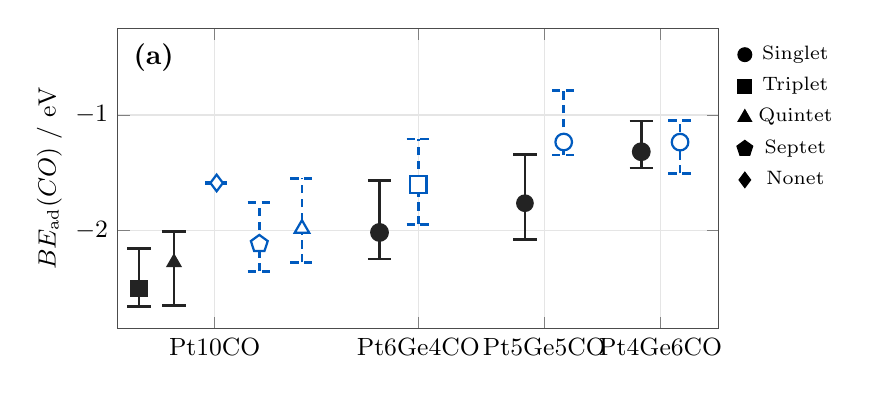
\begin{tikzpicture}
\begin{axis}[
  width=0.76\linewidth,
  height=5.4cm,
  xmin=0.45, xmax=3.55,
  ymin=-2.85, ymax=-0.25,
  xtick={0.95,2.00,2.65,3.25},
  xticklabels={\ce{Pt10CO},\ce{Pt6Ge4CO},\ce{Pt5Ge5CO},\ce{Pt4Ge6CO}},
  ylabel={$BE_{\rm ad}(\ce{CO})$ / eV},
  ylabel style={yshift=-2pt},
  tick label style={font=\small},
  label style={font=\small},
  grid=major,
  grid style={gray!20},
  axis line style={black!70},
  legend style={
    at={(1.02,0.98)},
    anchor=north west,
    draw=none,
    inner sep=2pt,
    row sep=1pt,
    font=\scriptsize,
    legend columns=1
  }
]
\addlegendimage{only marks,mark=*,mark size=2.5pt,black}
\addlegendentry{Singlet}
\addlegendimage{only marks,mark=square*,mark size=2.5pt,black}
\addlegendentry{Triplet}
\addlegendimage{only marks,mark=triangle*,mark size=2.8pt,black}
\addlegendentry{Quintet}
\addlegendimage{only marks,mark=pentagon*,mark size=3.0pt,black}
\addlegendentry{Septet}
\addlegendimage{only marks,mark=diamond*,mark size=2.8pt,black}
\addlegendentry{Nonet}
% Each vertical bar shows the minimum--maximum interval and each marker the
% mean over all Pt sites represented by the corresponding series. Horizontal
% offsets are used only for readability.
% Pt10der: triplet and quintet.
\addplot[ptten,line width=1.0pt] coordinates {(0.56,-2.657) (0.56,-2.156)};
\addplot[ptten,line width=1.0pt] coordinates {(0.50,-2.657) (0.62,-2.657)};
\addplot[ptten,line width=1.0pt] coordinates {(0.50,-2.156) (0.62,-2.156)};
\addplot[only marks,mark=square*,mark size=3.0pt,ptten] coordinates {(0.56,-2.501)};
\addplot[ptten,line width=1.0pt] coordinates {(0.74,-2.645) (0.74,-2.010)};
\addplot[ptten,line width=1.0pt] coordinates {(0.68,-2.645) (0.80,-2.645)};
\addplot[ptten,line width=1.0pt] coordinates {(0.68,-2.010) (0.80,-2.010)};
\addplot[only marks,mark=triangle*,mark size=3.0pt,ptten] coordinates {(0.74,-2.276)};
% Original Pt10 global-minimum parent: nonet, septet, and quintet.
\addplot[globalparent,densely dashed,line width=1.0pt] coordinates {(0.96,-1.595) (0.96,-1.580)};
\addplot[globalparent,densely dashed,line width=1.0pt] coordinates {(0.90,-1.595) (1.02,-1.595)};
\addplot[globalparent,densely dashed,line width=1.0pt] coordinates {(0.90,-1.580) (1.02,-1.580)};
\addplot[only marks,mark=diamond*,mark size=3.0pt,globalparent,
  mark options={fill=white,draw=globalparent,line width=0.8pt}] coordinates {(0.96,-1.588)};
\addplot[globalparent,densely dashed,line width=1.0pt] coordinates {(1.18,-2.353) (1.18,-1.755)};
\addplot[globalparent,densely dashed,line width=1.0pt] coordinates {(1.12,-2.353) (1.24,-2.353)};
\addplot[globalparent,densely dashed,line width=1.0pt] coordinates {(1.12,-1.755) (1.24,-1.755)};
\addplot[only marks,mark=pentagon*,mark size=3.2pt,globalparent,
  mark options={fill=white,draw=globalparent,line width=0.8pt}] coordinates {(1.18,-2.114)};
\addplot[globalparent,densely dashed,line width=1.0pt] coordinates {(1.40,-2.275) (1.40,-1.547)};
\addplot[globalparent,densely dashed,line width=1.0pt] coordinates {(1.34,-2.275) (1.46,-2.275)};
\addplot[globalparent,densely dashed,line width=1.0pt] coordinates {(1.34,-1.547) (1.46,-1.547)};
\addplot[only marks,mark=triangle*,mark size=3.0pt,globalparent,
  mark options={fill=white,draw=globalparent,line width=0.8pt}] coordinates {(1.40,-1.982)};
% Pt6Ge4: atom-substitution singlet and GM triplet.
\addplot[crossedparent,line width=1.0pt] coordinates {(1.80,-2.246) (1.80,-1.567)};
\addplot[crossedparent,line width=1.0pt] coordinates {(1.74,-2.246) (1.86,-2.246)};
\addplot[crossedparent,line width=1.0pt] coordinates {(1.74,-1.567) (1.86,-1.567)};
\addplot[only marks,mark=*,mark size=3.2pt,crossedparent] coordinates {(1.80,-2.016)};
\addplot[globalparent,densely dashed,line width=1.0pt] coordinates {(2.00,-1.947) (2.00,-1.207)};
\addplot[globalparent,densely dashed,line width=1.0pt] coordinates {(1.94,-1.947) (2.06,-1.947)};
\addplot[globalparent,densely dashed,line width=1.0pt] coordinates {(1.94,-1.207) (2.06,-1.207)};
\addplot[
  only marks,mark=square*,mark size=3.0pt,globalparent,
  mark options={fill=white,draw=globalparent,line width=0.8pt}
] coordinates {(2.00,-1.600)};
% Pt5Ge5: crossed parent and GM parent.
\addplot[crossedparent,line width=1.0pt] coordinates {(2.55,-2.076) (2.55,-1.342)};
\addplot[crossedparent,line width=1.0pt] coordinates {(2.49,-2.076) (2.61,-2.076)};
\addplot[crossedparent,line width=1.0pt] coordinates {(2.49,-1.342) (2.61,-1.342)};
\addplot[only marks,mark=*,mark size=3.0pt,crossedparent] coordinates {(2.55,-1.763)};
\addplot[globalparent,densely dashed,line width=1.0pt] coordinates {(2.75,-1.346) (2.75,-0.788)};
\addplot[globalparent,densely dashed,line width=1.0pt] coordinates {(2.69,-1.346) (2.81,-1.346)};
\addplot[globalparent,densely dashed,line width=1.0pt] coordinates {(2.69,-0.788) (2.81,-0.788)};
\addplot[only marks,mark=*,mark size=3.0pt,globalparent,
  mark options={fill=white,draw=globalparent,line width=0.8pt}] coordinates {(2.75,-1.234)};
% Pt4Ge6: crossed parent and GM parent.
\addplot[crossedparent,line width=1.0pt] coordinates {(3.15,-1.459) (3.15,-1.052)};
\addplot[crossedparent,line width=1.0pt] coordinates {(3.09,-1.459) (3.21,-1.459)};
\addplot[crossedparent,line width=1.0pt] coordinates {(3.09,-1.052) (3.21,-1.052)};
\addplot[only marks,mark=*,mark size=3.2pt,crossedparent] coordinates {(3.15,-1.318)};
\addplot[globalparent,densely dashed,line width=1.0pt] coordinates {(3.35,-1.506) (3.35,-1.046)};
\addplot[globalparent,densely dashed,line width=1.0pt] coordinates {(3.29,-1.506) (3.41,-1.506)};
\addplot[globalparent,densely dashed,line width=1.0pt] coordinates {(3.29,-1.046) (3.41,-1.046)};
\addplot[only marks,mark=*,mark size=3.0pt,globalparent,
  mark options={fill=white,draw=globalparent,line width=0.8pt}] coordinates {(3.35,-1.235)};
\node[anchor=north west,font=\bfseries] at (rel axis cs:0.01,0.98) {(a)};
\end{axis}
\end{tikzpicture}

\caption{Ranges and mean values of $BE_{\rm ad}(\ce{CO})$. Solid black
intervals and filled symbols represent the derivative
series, whereas dashed blue intervals and open symbols represent
calculations initiated from the reported GM structures. Each interval
spans the minimum-to-maximum $BE_{\rm ad}(\ce{CO})$ for one composition
and multiplicity, and the central symbol marks the mean over the sampled
Pt sites. Horizontal offsets are used only to separate overlapping
series.}
\label{fig:tfg_adsorption_distribution}
\end{figure}

For the \ce{Pt10^{der}CO} the \ce{CO} bound at site 6 reaches
the most strongly bound minimum, whereas those initiated at sites 1 and
9 converge to the same weakest minimum.  The ten Pt sites give a mean binding energy of $-2.50$ eV, and the
seven unique minima span
$-2.66$ to $-2.16$ eV. For the quintet state of bare \ce{Pt10} 
the ten Pt sites  mean  $BE_{\rm ad}(\ce{CO})$ is
$-2.28$ eV and their five unique minima span from $-2.65$ to $-2.01$ eV.

\red{In the \ce{Pt10^{GM}CO} series, the nonet carbonyls bind weakly and
span a narrow range ($-1.60$ to $-1.58$ eV). The septet and quintet
sets span from $-2.35$ to $-1.76$ eV and from $-2.28$ to $-1.55$ eV,
respectively.

The nonet values are much less negative than the global-minimum
\ce{Pt10}--\ce{CO} binding energy reported by Ugartemendia
\textit{et al.}\cite{ugartemendia:2022}. This difference arises from the
reference used for $BE_{\rm ad}(\ce{CO})$. Here, each nonet carbonyl is
referenced to the bare nonet cluster obtained by removing \ce{CO} and
reoptimizing from that carbonyl geometry. These values therefore describe
the nonet adsorption pathways sampled from \ce{Pt10^{GM}}. In the earlier
work, the association energy was obtained from the lowest \ce{Pt10} and
\ce{Pt10CO} structures on their respective potential-energy surfaces, so
it corresponds to the global-minimum pair rather than to these individual
pathways.}

To compare the two \ce{Pt10} structures at the same multiplicity, we also
calculated the quintet series for \ce{Pt10^{der}} and \ce{Pt10^{GM}}
(note that \ce{Pt10^{der}} quintet is 1.17 eV higher in energy than \ce{Pt10^{GM}} quintet).
The \ce{Pt10^{der}} quintet gives a mean binding energy of \(-2.28\) eV, whereas the \ce{Pt10^{GM}} quintet gives \(-1.98\) eV. Thus, within the same nominal spin state, the two structures differ by \(0.29\) eV in mean \(\ce{CO}\) binding energy. This result shows that the starting \(\ce{Pt10}\) structure can substantially change the CO-binding energies obtained for the different Pt sites.
The difference reflects the different local Pt environments and relaxation
pathways available from the two starting structures.

For the \ce{Pt_xGe_{10-x}^{der}CO} series ($x=6,5,4$), the mean
$BE_{\rm ad}(\ce{CO})$ becomes progressively less negative as the Ge
content increases, as shown in Figure~\ref{fig:tfg_adsorption_distribution}.
The binding energies vary between Pt sites, especially for
\ce{Pt5Ge5^{der}CO}, whose values span $0.73$ eV. Increasing the Ge
content therefore weakens \ce{CO} adsorption on average, in agreement
with earlier Pt--Ge studies.\cite{ugartemendia:2021,ugartemendia:2022}

The GM-based \ce{Pt_xGe_{10-x}CO} series, shown as dashed blue data in
Figure~\ref{fig:tfg_adsorption_distribution}, uses the multiplicity of the
corresponding bare-cluster GM: triplet for \ce{Pt6Ge4^{GM}} and singlet for
\ce{Pt5Ge5^{GM}} and \ce{Pt4Ge6^{GM}}. The effect of the GM structure
depends on composition. The \ce{Pt5Ge5^{GM}CO} series shifts toward weaker
adsorption, whereas the \ce{Pt4Ge6^{GM}CO} range is similar to that of
\ce{Pt4Ge6^{der}CO}. The \ce{Pt6Ge4^{GM}CO} series also gives weaker binding energies than the corresponding derivative series.

Taken together, the \ce{Pt_xGe_{10-x}^{der}CO} series shows a progressive
weakening of the mean \ce{CO} adsorption as the Ge content increases, while
the individual site values remain widely distributed. The GM-based
calculations show that the adsorption range can also shift by several tenths
of an eV when the starting structure and multiplicity change.

The following sections examine the local structural descriptors and the
energy contributions associated with cluster and \ce{CO} reorganization.
